%\chapter{Ensemble Methods}
%\label{ch:ensemblemethods}
\section{Evolving Stream Experimental Setting}
\label{sec:expsetting}
%Advanced analysis of data streams is quickly becoming
%a key area of data mining research as the number of applications
%demanding such processing increases.
%Online mining when such data streams evolve over time,
%that is when concepts drift or change completely,
%is becoming one of the core issues.
%When tackling non-stationary concepts, ensembles of classifiers
%have several advantages over single classifier methods:
%they are easy to scale and parallelize, they can adapt to change
%quickly by pruning under-performing parts of the ensemble, and they
%therefore usually also generate more accurate concept descriptions.
This section proposes a new experimental data stream framework for
studying concept drift using MOA. %, and two new  variants of Bagging.
%Using this new experimental framework,
%an evaluation study
%on synthetic and real-world datasets comprising up to ten
%million examples shows that the new
%ensemble methods perform very well compared to several known methods.
%
%\section{Introduction}
\BEGINOMIT
Conventional knowledge discovery tools assume that the volume of data is such 
that we can store all data in memory or local secondary storage, and there is no limitation on processing time. 
In the {\em Data Stream} model, we have space and time restrictions. Examples of data 
streams are sensoring video streams, network event logs, telephone call records,
credit card transactional flows, etc. 
An important fact is that data may be evolving over time, so we need methods
that adapt automatically. 

The following constraints apply in the Data Stream model:
\begin{enumerate}
\item  Data arrives as a potentially infinite sequence. Thus, it is impossible
 to store it all. Only a small summary can be computed and stored. %, and the rest 
%of the information thrown away. %Even if the information could be stored, 
%it would be infeasible to go over it for further processing.
\item The speed of arrival is fast, so that each particular element has to be 
processed essentially in real time, and then discarded.
\item The distribution generating the items may change over time. Thus, data from 
the past may become irrelevant (or even harmful) for the current prediction.
\end{enumerate}
%Under the Data Stream constraints, 
%The following constraints apply 
%In the Data Stream model,
%data arrives as a potentially infinite sequence, speed of arrival is fast, and 
%the distribution generating the items may change over time. 
Under the constraints of the Data Stream model,
the main properties of an ideal classification method %for mining data streams 
are the following:
high accuracy and fast adaption to change,
low computational cost in both space and time,
theoretical performance guarantees, 
and minimal number of parameters.

These properties may be interdependent: adjusting the time and space used 
by an algorithm can influence accuracy. By storing more pre-computed information, 
such as look up tables, an algorithm can run faster at the expense of
space. An algorithm can also run faster by processing less information, either
by stopping early or storing less, thus having less data to process. The more
time an algorithm has, the more likely it is that accuracy can be
increased.
\ENDOMIT
%Ensemble methods are combinations of several models whose individual predictions 
%are combined in some manner (e.g., averaging or voting) to form a final
%prediction.  Ensemble learning classifiers often have better accuracy and they are easier
%to scale and parallelize than single classifier methods.
A majority of concept drift research in data streams mining is done using
traditional data mining frameworks such as WEKA~\cite{weka}. As the data stream 
setting has constraints that a traditional data mining environment does not, 
we believe that MOA will help to improve the empirical
evaluation of these methods. 

%We present in Section~\ref{frame} a novel framework for evaluation 
%of concept drift. Sections~\ref{hast} and \ref{exp} present two novel ensemble methods
% for handling concept drift,  and a  first comprehensive cross-method comparison. 
%We present conclusions in Section~\ref{discussion}.
%
%{\em Repeatability:} %In accordance to the conference's guideline, the
%source code and executable
%versions of the software, as well as all datasets, will be available from
%MOA's homepage.
%Source code and datasets will be made available at 
%{\tt http://sourceforge.net/projects/moa-datastream}.

In data stream mining, we are interested in three main dimensions:
\begin{itemize}
 \item accuracy 
 \item amount of space necessary or computer memory
 \item the time required to learn from training examples and to predict
\end{itemize}

These properties may be interdependent: adjusting the time and space used 
by an algorithm can influence accuracy. By storing more pre-computed information, 
such as look up tables, an algorithm can run faster at the expense of
space. An algorithm can also run faster by processing less information, either
by stopping early or storing less, thus having less data to process. The more
time an algorithm has, the more likely it is that accuracy can be
increased.

In evolving data streams we are concerned about 

\begin{itemize}
 \item evolution of accuracy
 \item probability of false alarms
 \item probability of true detections
 \item average delay time in detection
\end{itemize}

Sometimes, learning methods do not have change detectors implemented inside,
and then it may be hard to define ratios of false positives and negatives, and
average delay time in detection. In these cases, learning curves may be a useful 
alternative for observing the evolution of accuracy in changing environments.
%or errors when change occurs.

%Under the constraints of the Data Stream model,
To summarize, the main properties of an ideal learning method for mining evolving data streams 
are the following:
high accuracy and fast adaption to change,
low computational cost in both space and time,
theoretical performance guarantees, 
and minimal number of parameters. 


\BEGINOMIT
\section{Experimental framework for concept drift}
\label{sec:expframe}

A data stream environment has different requirements from the traditional 
setting~\cite{Kirkby-PhD}. The most significant are the following: 
\begin{description}
\item[Requirement 1] Process an example at a time, and inspect
 it only once (at most)
\item[Requirement 2] Use a limited amount of memory
\item[Requirement 3] Work in a limited amount of time
\item[Requirement 4] Be ready to predict at any time
\end{description}
\begin{figure}[t]
\begin{center} 
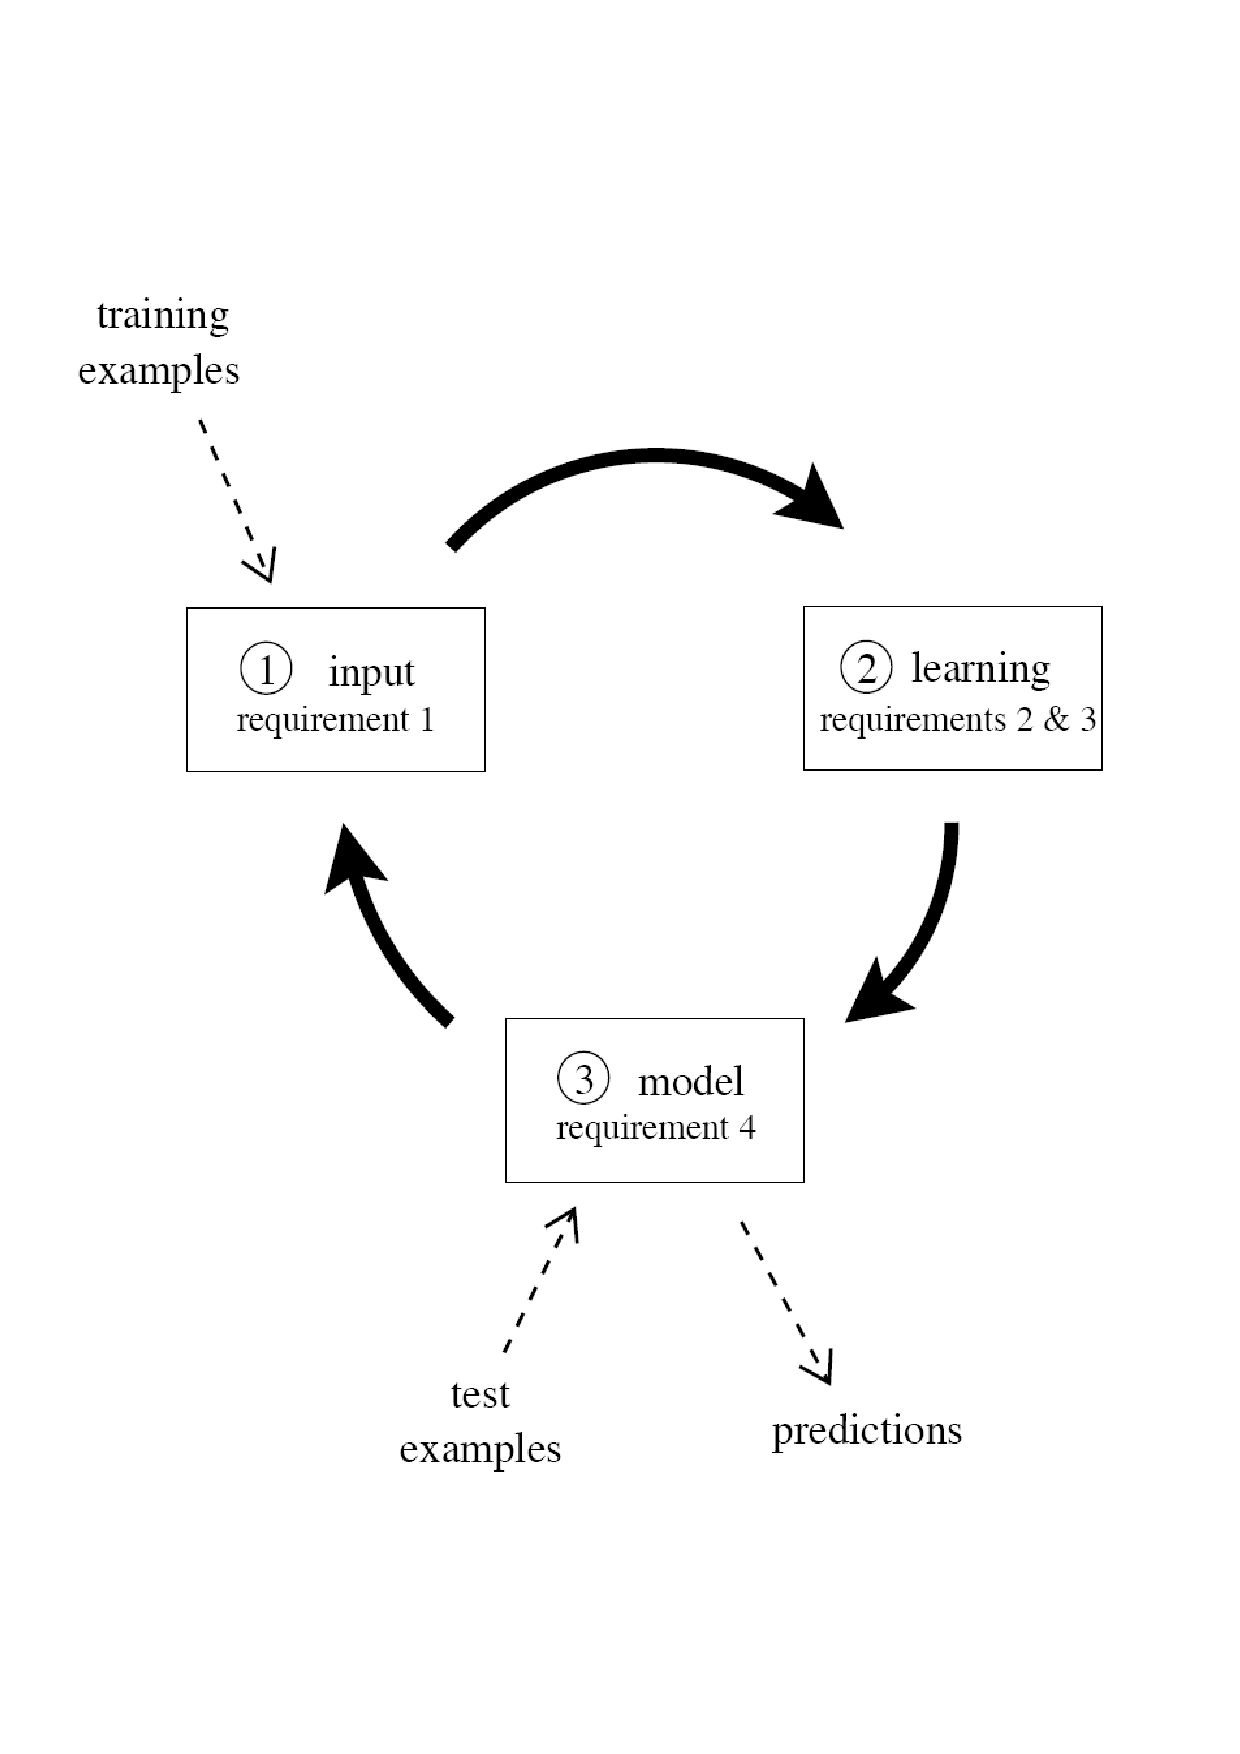
\epsfig{file=Frame, scale=.18}
\end{center} 
\caption{The data stream classification cycle}
\label{fig:cycle}
\end{figure} 
We have to consider these requirements in order to design a new experimental
framework for data streams.
Figure~\ref{fig:cycle} illustrates the typical use of a data stream 
classification algorithm, and how the requirements fit %in. The general model 
%of data stream classification follows these three steps 
in a repeating cycle:
\begin{enumerate}
\item  The algorithm is passed the next available example from the stream
   (requirement 1).
\item  The algorithm processes the example, updating its data structures. It
   does so without exceeding the memory bounds set on it (requirement 2),
   and as quickly as possible (requirement 3).
\item  The algorithm is ready to accept the next example. On request it is
   able to predict the class of unseen examples
   % , and  supply a model that can be used to  
   (requirement 4).
\end{enumerate}


In traditional batch learning the problem of limited data is overcome
by analyzing and averaging multiple models produced with different random
arrangements of training and test data. In the stream setting the problem of
(effectively) unlimited data poses different challenges. One solution involves
taking snapshots at different times during the induction of a model to see how
much the model improves.

The evaluation procedure of a learning algorithm determines which examples
are used for training the algorithm, and which are used to test the model output
by the algorithm. The procedure used historically in batch learning has partly
depended on data size. As data sizes increase, practical
time limitations prevent procedures that repeat training too many times. It is
commonly accepted with considerably larger data sources that it is necessary
to reduce the numbers of repetitions or folds to allow experiments to complete
in reasonable time. 
    When considering what procedure to use in the data stream setting, one of
the unique concerns is how to build a picture of accuracy over time. Two main
approaches arise~\cite{Kirkby-PhD}:
\begin{itemize}
 \item {\bf Holdout}:
When traditional batch learning reaches a scale where cross-validation is too time 
consuming, it is often accepted to instead measure performance on a single holdout
set. This is most useful when the division between train and test sets have
been pre-defined, so that results from different studies can be directly compared. 
%Viewing data stream problems as a large-scale case of batch learning,
%it then follows from batch learning practices that a holdout set is appropriate.
\item {\bf Interleaved Test-Then-Train}:
 Each individual example can be used to test the model
before it is used for training, and from this the accuracy can be incrementally
updated. When intentionally performed in this order, the model is always
being tested on examples it has not seen. This scheme has the advantage that
no holdout set is needed for testing, making maximum use of the available
data. It also ensures a smooth plot of accuracy over time, as each individual
example will become increasingly less significant to the overall average.
%    With this procedure the statistics are updated with every example in the
%stream, and can be recorded at that level of detail if desired. For efficiency
%reasons a sampling parameter can be used to reduce the storage requirements
%of the results, by recording only at periodic intervals like the holdout method.
\end{itemize}
   As data stream classification is a relatively new field, such evaluation 
practices are not nearly as well researched and established as they are
in the traditional batch setting. 
The majority of experimental evaluations use less than one million
training examples. Some papers use more than this, up to ten million examples,
and only very rarely is there any study like Domingos and 
Hulten~\cite{Domingos,hulten-mining}  that is in the order of tens of millions 
of examples. In the context of data streams this is disappointing, because to be
truly useful at data stream classification the algorithms need to be capable of 
handling very large (potentially infinite) streams of examples. Demonstrating 
systems only on small amounts of data does not build a convincing case for capacity
to solve more demanding data stream applications.
%    There are several possible reasons for the general lack of training data for
%evaluation. It could be that researchers come from a traditional machine learning 
%background with entrenched community standards, where results involving
%cross-validation on popular real-world data sets are expected for credibility,
%and alternate practices are less understood. Emphasis on using real-world
%data will restrict the sizes possible, because there is very little data 
%freely available that is suitable for data stream evaluation.
%Another reason could be that the methods are being directly compared with
%batch learning algorithms, as several of the papers do, so the sizes may 
%deliberately be kept small to accommodate batch learning. Hopefully no evaluations
%are intentionally small due to proposed data stream algorithms being too slow
%or memory hungry to cope with larger amounts of data in reasonable time or
%memory, because this would raise serious doubts about the algorithm's
%practical utility.
\ENDOMIT
\BEGINOMIT
    A claim of~\cite{Kirkby-PhD} is that in order to adequately evaluate data stream
classification algorithms they need to be tested on large streams, in the order
of tens of millions of examples where possible, and under explicit memory
limits. Any less than this does not actually test algorithms in a realistically
challenging setting. 
\ENDOMIT

\subsection{Concept Drift Framework}
We present the new experimental framework for concept drift in MOA. Our goal was to introduce
artificial drift to data stream generators in a straightforward way. 
 
The framework approach most similar to the one presented in this Chapter 
 is the one proposed by Narasimhamurthy et al.~\cite{kuncheva07}.
They proposed a general 
framework to generate data simulating
changing environments. Their framework accommodates the %currently favourite 
STAGGER and Moving Hyperplane generation
strategies. % and offers a versatile approach towards
%devising new strategies.
They consider a set of $k$ data sources with known distributions.
As these distributions at the sources are fixed, the data distribution
at time $t$, $D^{(t)}$ is specified through $v_i(t)$, where 
 $v_i(t) \in [0,1]$ specify the extent of the influence of data
source $i$ at time $t$:
$$D^{(t)} = \{v_1(t), v_2(t), \ldots, v_k(t) \}, \sum_{i} v_i(t)= 1$$
Their framework covers gradual and abrupt changes.
Our approach is more concrete, %general,
we begin by dealing 
with a simple scenario: a data stream and two different concepts. Later, we will 
consider the general case with more than one concept drift { events}. 

Considering data streams as data generated from pure distributions, we can model
a concept drift { event} as a weighted combination %a mixture distribution, 
of two pure distributions that characterizes the target concepts before and after
the drift. In our framework, we need to define the probability that every new 
instance of the stream belongs to the new concept after the drift. We will use 
the sigmoid function, as an elegant and practical solution.

\begin{figure}
\begin{tikzpicture}[domain=-2:9]
  \draw[step=2,very thin,color=gray] (-0.1,-0.1) grid (8.2,4.2);
  \draw[->] (-2.2,0) -- (8.2,0) node[right] {$t$};
  \draw[->] (0,-0.2) -- (0,4.2) node[above] {$f(t)$};
  \draw[<->] (2,-0.6) -- (6,-0.6) node[below] {};
  \draw[color=blue!50!black, domain=2:6] plot[id=x]   function{(x-2)}           node[right]{}; %{$f(x) =x$};
  %\draw[color=blue]   plot[id=sin] function{sin(x)}       node[right] {$f(x) = \sin x$};
  \draw[color=red!50!black] plot[id=exp] function{4/(1+exp(4-x))} node[right] {$f(t)$};% = 1/{(1+ \mathrm e^{-s (x-x_0)}})$};
  %\shadedraw[left color=gray,right color=green, draw=green!50!black] (2,0) -- (2.5,0) arc (0:45:.5) -- cycle; 
  \colorlet{anglecolor}{blue!50!black}
  \filldraw[fill=blue!20,draw=anglecolor] (2,0) -- (2.5,0) arc(0:45:.5);
  \draw (2.7,.3) node[anglecolor] {$\alpha$};
  \filldraw[fill=blue!20,draw=anglecolor] (4,2) -- (4.5,2) arc(0:45:.5);
  \draw (4.7,2.3) node[anglecolor] {$\alpha$};

  \draw (4,-0.3) node[] {$t_0$};
  \draw (4,-0.9) node[] {$W$};
  \draw (-0.5,2) node[] {$0.5$};
  \draw (-0.5,4) node[] {$1$};

\end{tikzpicture}
\caption{A sigmoid function $f(t) = 1/{(1+ \mathrm e^{-s (t-t_0)}})$.}
\label{fig:ConceptChange}
\end{figure}
We see from Figure~\ref{fig:ConceptChange} that the sigmoid function 
$$f(t) = 1/{(1+ \mathrm e^{-s (t-t_0)}})$$
has a derivative at the point $t_0$ equal to $f'(t_0) = s/4$. The tangent of angle 
$\alpha$ is equal to this derivative, $\tan \alpha = s/4$. We observe that 
$ \tan \alpha = 1/ W$,
and as $s= 4 \tan \alpha$ then $s=4/W$. So the parameter $s$ in the sigmoid 
gives the length of $W$ and the angle $\alpha$. 
In this sigmoid model we only need to specify two parameters : 
$t_0$ the point of change, and $W$ the length of change.
Note that $$f(t_0+\beta \cdot W)=1 -f(t_0-\beta \cdot W),$$ and  that $f(t_0+\beta \cdot W)$ and $f(t_0-\beta \cdot W)$ 
are constant values that don't depend on $t_0$ and $W$: 
$$f(t_0+W/2) = 1 - f(t_0-W/2) = 1/( 1+ e^{-2}) \approx 88.08 \%$$  
$$f(t_0+W) = 1 - f(t_0-W) = 1/( 1+ e^{-4}) \approx 98.20 \%$$  
$$f(t_0+2W) = 1 - f(t_0-2W) = 1/( 1+ e^{-8}) \approx 99.97 \%$$
\begin{definition} %{\bf ($\oplus$-operation)}\\
Given two data streams $a$, $b$, we define $c = a  \oplus^{W}_{t_0} b$ as the 
data stream built joining the two data streams $a$ and $b$, where
$t_0$ is the point of change, $W$ is the length of change and 
\begin{itemize}
 \item $\Pr[ c(t) = a(t)] = \mathrm e^{-4(t-t_0)/W}/{(1+ \mathrm e^{-4(t-t_0)/W})}$
 \item $\Pr[ c(t) = b(t)] = 1/{(1+ \mathrm e^{-4(t-t_0)/W})}$.
\end{itemize}
\end{definition}
We observe the following properties, if $a \ne b$:
\begin{itemize}
 \item $a \oplus^{W}_{t_0} b \neq b \oplus^{W}_{t_0} a$
 \item $a \oplus^{W}_{t_0} a = a$
 \item $a \oplus^{0}_{0} b = b$
 \item $a \oplus^{W}_{t_0} ( b \oplus^{W}_{t_0} c) \neq (a \oplus^{W}_{t_0}  b)
	 \oplus^{W}_{t_0} c$
 \item $a \oplus^{W}_{t_0} ( b \oplus^{W}_{t_1} c) \approx (a \oplus^{W}_{t_0}  b)
	 \oplus^{W}_{t_1} c$ if $t_0<t_1$ and $W \ll |t_1-t_0|$
\end{itemize}
In order to create a data stream with multiple concept changes, we can build new 
data streams joining different concept drifts:
$$( ( (a \oplus^{W_0}_{t_0}  b) \oplus^{W_1}_{t_1} c) \oplus^{W_2}_{t_2} d ) \ldots $$ 

%and, in the case that all $W$'s are equal

%$$( ( (a \oplus^{W}_{t_0}  b) \oplus^{W}_{t_1} c) \oplus^{W}_{t_2} d ) \ldots $$ 

\subsection{Datasets for concept drift}
\label{datasets}
Synthetic data has several advantages \--- it is easier to reproduce and there is 
little cost in terms of storage and transmission. For this framework, 
the data generators most commonly found in the literature have been collected.

\begin{description} %\subsubsection{SEA Concepts}
 \item[SEA Concepts Generator] This dataset contains abrupt concept drift, 
first introduced  in~\cite{sea}. It is generated using three attributes,
where only the two first attributes are relevant. 
All three attributes have values between 0 and 10.
The points of the dataset are divided into $4$ blocks with different concepts. 
In each block,  the classification is done using $f_1+ f_2 \leq \theta$, 
where $f_1$ and $f_2$ represent the first two attributes 
and $\theta$ is a threshold value. 
The most frequent values are 9, 8, 7 and 9.5 for the data blocks. 
In our framework, SEA concepts are defined as follows:
$$( ( (SEA_9 \oplus^{W}_{t_0}  SEA_8) \oplus^{W}_{2t_0} SEA_7) \oplus^{W}_{3t_0} SEA_{9.5} )  $$ 
 \item[STAGGER Concepts Generator] %\subsubsection{STAGGER Concepts}
%The STAGGER Concepts
They were introduced by Schlimmer and Granger in~\cite{SchlimmerG86}.
The concept description in STAGGER is a collection of elements, where each 
individual element is a Boolean function of attribute-valued pairs that is 
represented by a disjunct of conjuncts. A typical example of a concept description
covering either green rectangles or red triangles can be represented by (shape 
rectangle and colour green) or (shape triangles and colour red).
 \item[Rotating Hyperplane]%\subsubsection{Hyperplane}
%Another frequently used dataset is 
%The rotating hyperplane, 
This dataset was used as testbed for CVFDT 
versus VFDT in~\cite{hulten-mining}. A hyperplane in $d$-dimensional space is the
set of points $x$ that satisfy $$ \sum^{d}_{i=1} w_i x_i = w_0 = \sum^{d}_{i=1} w_i  $$
where $x_i$, is the ith coordinate of $x$. Examples for which $ \sum^{d}_{i=1} w_i x_i \ge w_0 $  
are labeled positive, and examples for which  $ \sum^{d}_{i=1} w_i x_i < w_0 $
are labeled negative. 
Hyperplanes are useful for simulating time-changing concepts, because we can
change the orientation and position of the hyperplane in a
smooth manner by changing the relative size of the weights.
We introduce change to this dataset adding drift to each weight attribute 
 $w_i = w_i + d\sigma$,
where $\sigma$ is the probability that the direction of change is reversed and $d$ is
the change applied to every example.
\item[Random RBF Generator]%\subsubsection{Random RBF Generator}
{ This generator was devised to offer an alternate complex concept type that is not 
straightforward to approximate with a decision tree model.}
%This generator was devised to offer an alternate concept type that is not 
%necessarily as easy to capture with a decision tree model.
The RBF (Radial Basis Function) generator works as follows: A fixed number
of random centroids are generated. Each center has a random position,
a single standard deviation, class label and weight. New examples are 
generated by selecting a center at random, taking weights into consideration so
that centers with higher weight are more likely to be chosen. A random 
direction is chosen to offset the attribute values from the central point. The
length of the displacement is randomly drawn from a Gaussian distribution
with standard deviation determined by the chosen centroid. The chosen 
centroid also determines the class label of the example. This effectively creates a
normally distributed hypersphere of examples surrounding each central point
with varying densities. Only numeric attributes are generated. 
Drift is introduced by moving the centroids with constant speed. This speed is
initialized by a drift parameter.
\BEGINOMIT
 \item[LED Generator]%\subsubsection{LED Generator}
This data source originates from the CART book~\cite{cart93}. An implementation in
C was donated to the UCI~\cite{uci} machine learning repository by David Aha. The
goal is to predict the digit displayed on a seven-segment LED display, where
each attribute has a 10\% chance of being inverted. It has an optimal Bayes
classification rate of 74\%. The particular configuration of the generator used
for experiments (led) produces 24 binary attributes, 17 of which are irrelevant.
 \item[Waveform Generator]%\subsubsection{Waveform Generator}
It shares its origins with { LED}, and was also donated by David Aha
to the UCI repository. The goal of the task is to differentiate between three
different classes of waveform, each of which is generated from a combination
of two or three base waves. The optimal Bayes classification rate is known
to be 86\%. There are two versions of the problem, wave21 which has 21 numeric
attributes, all of which include noise, and wave40 which introduces an additional 19
irrelevant attributes.
 \item[Function Generator] %subsubsection{Function Generator}
It was introduced by Agrawal et al. in~\cite{agrawal}, and was a common
source of data for early work on scaling up decision tree learners~\cite{dbmine,sliq, sprint,rainforest}.
The generator produces a stream containing nine attributes, six numeric and 
three categorical. Although not explicitly stated by the authors, a sensible 
conclusion is that these attributes describe hypothetical loan applications.
There are ten functions defined for generating binary class labels from the
attributes. 
Presumably these determine whether the loan should be approved. 
\ENDOMIT
 \end{description}
Data streams may be considered infinite sequences of $(x,y)$ where $x$ is the feature vector and $y$
the class label. Zhang et al.~\cite{Zhang08} observe that $ p(x,y) = p(x|t) \cdot p(y|x) $ and categorize concept drift in two types:
\begin{itemize}
 %\item 
\item \emph{Loose Concept Drifting (LCD)} when concept drift is caused only by the change of the class prior probability $p(y|x)$, %\item 
\item  \emph{Rigorous Concept Drifting (RCD)} when concept drift is caused by the change of the class prior probability $p(y|x)$ and the conditional probability $p(x|t)$  
\end{itemize}

Note that the Random RBF Generator has RCD drift, and the rest of the dataset generators have LCD drift.

\subsubsection{Real-World Data}


%The first place to find real-world benchmark data for evaluating machine learning 
%algorithms is the UCI machine learning repository~\cite{Adult}. Larger real-world
%data sets can be found in the UCI KDD archive~\cite{UCIKDD}, which was established to
%serve the needs of larger scale benchmarking.

%The data set with the most examples is KDD Cup 1999 which has nearly
%five million training examples. The task is to detect network intrusion attempts. 
%After initial experiments with this data it became clear that it is not
%a very useful benchmark-it is too easy to achieve near-perfect accuracy, there
%are many classes with a highly imbalanced distribution of examples between
%classes, making it hard to discern anything from the accuracies measured for
%competing methods.
It is not easy to find large real-world datasets
for public benchmarking, especially with substantial concept change. %big real-world datasets.
The UCI machine learning repository~\cite{uci} contains some real-world benchmark 
data for evaluating machine learning techniques. 
We will consider three : Forest Covertype, Poker-Hand, and Electricity.
%algorithms is the UCI machine learning repository~\cite{Adult}.
%In the experiments with  real datasets we use two UCI 
%datasets~\cite{Adult} Adult and Poker-Hand from the UCI repository of machine learning databases.
\begin{description}
 \item[Forest Covertype dataset] It contains 
the forest cover type for 30 x 30 meter cells obtained from US Forest Service (USFS) Region 2 Resource Information System (RIS) data. 
It contains $581,012$ instances and $54$ attributes, and
it has been used
in several papers on data stream classification~\cite{vfdtc, ozaexp}.
 \item[Poker-Hand dataset] %The Poker-Hand dataset 
It consists of $1,000,000$ %1,025,010 
instances and $11$ attributes.
Each record of the Poker-Hand dataset is an example of a hand consisting of five playing cards drawn from a standard deck of $52$. Each card is described using two attributes (suit and rank), for a total of $10$ predictive attributes. There is one Class attribute that describes the ``Poker Hand''. The order of cards is important, which is why there are $480$ possible Royal Flush hands instead of $4$.
\item[Electricity dataset] 
Another widely used dataset is the Electricity Market Dataset described by M. Harries \cite{Harries} 
and used by Gama \cite{Gama}. 
This data was collected from the Australian New South Wales Electricity Market. 
In this market, the prices are not fixed and are affected by demand and supply of the market. 
The prices in this market are set every five minutes. 
The ELEC2 dataset contains $45,312$ instances. %dated from $7$ May $1996$ to $5$ December $1998$. 
Each example of the dataset refers to a period of $30$ minutes, i.e. there are $48$ instances
for each time period of one day. %Each example on the dataset has 5 fields, the
%day of week, the time stamp, the NSW electricity demand, the Vic electricity
%demand, the scheduled electricity transfer between states and the class label.
The class label identifies the change of the price related to a moving average of
the last $24$ hours. The class level only reflect deviations of the price on a one
day average and removes the impact of longer term price trends. 
 \end{description}
 
The size of these datasets is small, compared to tens of millions of training examples of synthetic datasets: $45,312$ for ELEC2 dataset, $581,012$ for CoverType, and $1,000,000$ for Poker-Hand.
Another important fact is that we do not know when drift occurs or if there is any drift. We may simulate RCD concept drift, joining the three datasets, merging attributes, and supposing that each dataset corresponds to a different concept.
$$ \textrm{CovPokElec} =  (\textrm{CoverType} \oplus^{5,000}_{581,012} \textrm{Poker}) \oplus^{5,000}_{1,000,000} \textrm{ELEC2} $$ 

%For the style of evaluation required by this paper, where several hundreds
%of millions of training examples are required to test genuine ability to handle
%data streams, these data sets are simply not adequate. The need to rely on
%artificial data is unfortunate but necessary.
\BEGINOMIT
\subsection{MOA Experimental Framework}
\label{ssec:moa}
{\bf M}assive {\bf O}nline {\bf A}nalysis (MOA)~\cite{MOA} is a
framework for online learning from continuous %supplies of examples, such as 
data streams.
The data stream evaluation framework and most of the classification algorithms evaluated in this thesis
were implemented in the Java programming language extending the MOA framework.
MOA includes a collection of offline and online methods as well as tools for evaluation. 
In particular, it implements boosting, bagging, and Hoeffding Trees, all %both 
with and without Na{\"\i}ve Bayes classifiers at the leaves. 
%MOA  graphical user interface is shown in Figure~\ref{fig:moagui}.
%However, a command line interface is also available.

%\begin{figure}[t]
%\begin{center} 
%\epsfig{file=MOATL, scale=0.3}
%\end{center} 
%\caption{MOA Graphical User Interface}
%\label{fig:moagui}
%\end{figure} 

MOA is related to WEKA, the Waikato
Environment for Knowledge Analysis~\cite{weka}, which is an award-winning open-source 
workbench containing implementations of a wide range of batch machine 
learning methods. WEKA is also written in Java. The main benefits
of Java are portability, where applications can be run on any platform with
an appropriate Java virtual machine, and the strong and well-developed support 
libraries. Use of the language is widespread, and features such as the
automatic garbage collection help to reduce programmer burden and error.

    One of the key data structures used in MOA is the description of an example
from a data stream. This structure borrows from WEKA, where an example is
represented by an array of double precision floating point values. This provides
freedom to store all necessary types of value \--- numeric attribute values can be
stored directly, and discrete attribute values and class labels are represented
by integer index values that are stored as floating point values in the array.
Double precision floating point values require storage space of 64 bits, or 8
bytes. This detail can have implications for memory usage. %utilization.
\ENDOMIT